% You should title the file with a .tex extension (hw1.tex, for example)
\documentclass[11pt]{article}

\usepackage{amsmath}
\usepackage{mathtools}
\usepackage{amssymb}
\usepackage{wrapfig}
\usepackage{fancyhdr}
\usepackage{tikz-qtree}
\usepackage{tikz-qtree-compat}
\usepackage[normalem]{ulem}
\usepackage{tikz}
\usepackage{graphicx}
\DeclareMathOperator*{\argmin}{argmin}
\DeclareMathOperator*{\argmax}{argmax}

\oddsidemargin0cm
\topmargin-2cm     %I recommend adding these three lines to increase the 
\textwidth16.5cm   %amount of usable space on the page (and save trees)
\textheight23.5cm  

\newcommand{\question}[2] {\vspace{.25in} \hrule\vspace{0.5em}
\noindent{\bf #1: #2} \vspace{0.5em}
\hrule \vspace{.10in}}
\renewcommand{\part}[1] {\vspace{.10in} {\bf (#1)}}
\linespread{1.5}

\newcommand{\myname}{Anonymous Authors}
\newcommand{\myhwnum}{12}

\setlength{\parindent}{0pt}
\setlength{\parskip}{5pt plus 1pt}
 
\DeclarePairedDelimiter\abs{\lvert}{\rvert}%

\pagestyle{fancyplain}

\begin{document}

\medskip                        % Skip a "medium" amount of space
                                % (latex determines what medium is)
                                % Also try: \bigskip, \littleskip

\thispagestyle{plain}
{\Large Statistical inference in theoretical models of cognition} \\
Sean R. Bittner, \textit{the DSN alliance}, John P. Cunningham
\section{Abstract}
Theoretical neuroscientists often design circuit models of neural activity with the hopes of producing some emergent property observed in data.  However, the standard inference toolkit is designed to condition on data points collected in an experiment, rather than the abstract notion of an emergent property.  We introduce a novel machine learning methodology called degenerate solution networks (DSNs), which learn a distribution of generative model parameterizations that produces the emergent property of interest, and is otherwise as random as possible.  We use DSNs to advance theoretical understanding of the stomatogastric ganglion (STG), primary visual cortex (V1), superior colliculus (SC), and low rank recurrent neural networks (RNNs).  As models continue to increase in complexity and become less tractable in terms of conventional analytic and theoretical approaches, DSNs will be a useful tool for theorists to interrogate their models

\section{Introduction}
Developing a theory for a neural computation requires a.) a parameterized model of the brain area(s) executing the computation, b.) a mathematical definition of the emergent properties of the model signifying the computation, and then c.) a characterization of the model parameters that produce these emergent properties.  Since the advent of theoretical neuroscience, parameterized models of neural systems (a) have become ubiquitous in neuroscience \cite{abbott2008theoretical}.  The emergent properties of interest (b) in these models is predicated by the nervous system function being studied.  Prevalent examples include biophysical circuit firing frequency (cite review), memory capacity (cite review), holistic response properties of sensory areas (cite a few), and task execution (cite a few).

In idealized practice of theory, scientists analytically derive parametric solutions to their model that produce the emergent property in focus (c).  These derivations often rely on modeling strategies from physics  (e.g. \cite{hopfield1984neurons, sompolinsky1988chaos}). 
% It is often necessary for theoretical neuroscientists to extend these approaches [cite], or build an entirely new theoretical approach [cite]. 
Unfortunately, such gold standard theoretical practices are not always feasible in neuroscience.  The desire to make a neural model more biologically realistic and interpretable is at odds with the tractability of its analysis.  In cases of such realistic modeling, theorists search for structure in simulated activity \cite{gutierrez2013multiple} (cite a bunch here).  This approach becomes computationally intractable as the number of parameters increases, and glaringly lacks a probabilistic treatment of parameter space.

Classically, the probabilistic treatment of model parameter spaces, statistical inference, is designed to condition on an experimentally observed set of data points.  This is appropriate in many scientific contexts, but is often unsuitable for theoretical neuroscience.  Contrary to the common narrative, theoreticians rarely attempt to directly reproduce experimental data.  They work with abstracted mathematical definitions of the requisite neural circuit properties for computation (albeit, these are motivated by experimental findings).  Thus, in practice, theoreticians want to condition their interpretable neural circuit models on the abstract notion of an emergent property of computation, \textit{not} a data set.  Here, we present a novel machine learning method, degenerate solution networks (DSNs), which are particularly useful for theoretical neuroscience research.  DSNs learn a distribution of theoretical model parameterizations that produces some statistically constrained behavior, and is otherwise as random as possible.  

DSNs are a tool designed for theorists, that enables a new class of model analyses relying on the full distribution of generative parameters that result in some statistically specified activity. In this study, we use DSNs to advance theory of interpretable models of neural computation ranging from biophysical conductance-based circuits to low-rank RNNs.  We begin by introducing the method along with an exploratory analysis of the stomatogastric ganglion (STG) circuit.  Then, we apply the same hessian analysis to an inhibitory subtype population model of primary visual cortex (V1) to characterize the possible strategies of inhibition stabilization.  By conditioning on task execution with DSNs, we are able to identify a sufficient mechanism of task learning in an interpretable model of superior colliculus, and characterize the role of chaos and limit cycle geometry in the stability of oscillating RNNs.  Equipped with this method, we readily attain novel insights into cutting-edge models, suggesting that DSNs should be an integral piece of technology for theoretical neursocience moving forward.

\section{Results}
\subsection{Degenerate solution networks}
We have a host of methods from Bayesian machine learning that prescribe how to go from data points through a likelihood model and choice of prior to a posterior distributions on likely parameterizations to have produced such data.  But, how do we condition on emergent properties of behavior that we prefer to define statistically?  DSNs combine ideas from likelihood-free variational inference (cite Tran et al) and maximum entropy flow networks (cite Gabe) to make this possible.  A maximum entropy flow network is used as a deep generative model for the parameter distribution of the theoretical model, while these samples are passed through a differentiable dynamics simulator, which can lack a tractable likelihood function.

Consider model parameterization $z$ and data $x$ generated from some theoretical model simulator represented as $p(x \mid z)$, which may be deterministic or stochastic.  Neural circuit models usually have known sampling procedures for simulating activity given a circuit parameterization, yet often lack an explicit likelihood function for the neural activity due to having nonlinear dynamics. DSNs learn a distribution on parameters $z$, that yields a behavior of interest $\mathcal{B}$,
\begin{equation}
\mathcal{B}: E_{z \sim q_\theta}\left[ E_{x\sim p(x \mid z)}\left[T(x)\right] \right] = \mu
\end{equation}
by making a deep generative approximation $q_\theta(z)$ to $p(z \mid \mathcal{B})$.  So, over the degenerate solution distribution $q_\theta(z)$ of the model for behavior $\mathcal{B}$, the emergent properties (or sufficient statistics) $T(x)$ are constrained in expectation to $\mu$.

 In deep generative models, a simple random variable $\omega \sim q_0$ is mapped deterministically via a function $f_\theta$ parameterized by a neural network to the support of the distribution of interest, where $z = f_{\theta}(\omega) = f_l(..f_1(\omega))$.  Given a theoretical model and some behavior of interest, DSNs (Fig. 1A) are trained by optimizing parameters $\theta$ to find the best approximation $q_{\theta}^*(z)$ within the deep generative variational family $Q$ to $p(z \mid \mathcal{B})$ by differentiating through a calculation of the emergent properties given the parameters.  This is done by maximizing the entropy of the learned distribution $q_{\theta}^*(z)$ such that the constraints in $\mathcal{B}$ are satisfied (Fig. 1B):

\[q_\theta^*(z) = \mathop{\arg\,\max}\limits_{q_\theta \in Q} H(q_\theta(z)) \]
\[ \text{s.t.  } E_{z \sim q_\theta}\left[ E_{x\sim p(x \mid z)}\left[T(x)\right] \right] = \mu \]


( -- paragraph about the STG -- )

\subsection{Exploratory analysis of a theoretical model}
Dynamical models with two populations (excitatory (E) and inhibitory (I) neurons) of visual processing have been used to reproduce a host of experimentally documented phenomena in V1.   When an inhibition stabilized network (ISN, the I population stabilizes an otherwise unstable E population), these models exhibit the paradoxical effect \cite{tsodyks1997paradoxical}, selective amplification \cite{murphy2009balanced}, surround suppression \cite{ozeki2009inhibitory}, and  sensory integrative properties \cite{rubin2015stabilized}.  Since I neurons mostly fall into one of three classes (parvalbumin (P)-, somatostatin (S)-, and vasointestinal peptide (V)-expressing neurons) \cite{markram2004interneurons, rudy2011three}, theorists look to extend these dynamical models to four populations \cite{litwin2016inhibitory}.  A current challenge in theoretical neuroscience is understanding the distributed role of inhibition stabilization across these subtypes.  

These four populations exhibit neuron-type specific connectivity (Fig. 1A) \cite{pfeffer2013inhibition}, in which some populations do not project to others.  Since S and V are the only populations that mutually inhibit each other, a popular conceptualization is that S and V have winner-take-all dynamics.  In fact, evidence in mice suggests that V silences S when presented with large stimuli, and S silences V for small stimuli \cite{dipoppa2018vision}.  Here, we use DSNs to understand the possible sources of inhibition stabilization in this V1 model, when either S or V is inactive.  The behavior of the DSN distributed models are constrained to produce two things: 1.) a mean-zero distribution of ISN coefficients $\gamma(W) = 1 - f^{'}(f^{-1}(r_E(W)))W_{EE}$ with some variance, and 2.) $\alpha$-population silencing $r_\alpha(W) = 0$, for $\alpha \in \{ S, V \}$ (Fig. 1B).  When $\gamma < 0$ the network is ISN, and not ISN otherwise.  Constraining the DSN behavior to a zero-mean distribution of ISN coefficients gives us samples of both ISN and non-ISN networks, optimizied to have greatest variety of stabilization motifs.

When optimized to produce a variety of stabilization motifs, there are informative differences between S-silenced and V-silenced DSN posteriors.  The marginal posteriors for each weight matrix element ($W_{EE}$ is fixed to 1.0, and $W_{*E}$ is one parameter), are visualized by their location in the dynamics matrix (Fig. 1C).  Low-variance marginals, like $q_\theta(W_{PP} \mid \mathcal{B}_{S=0})$, $q_\theta(W_{VP} \mid \mathcal{B}_{S=0})$, and $q_\theta(W_{SV} \mid \mathcal{B}_{S=0})$, indicate that either the $\gamma(W)$, S-silencing, or both are sensitive to changes in such parameters.  Whereas, $q_\theta(W_{PP} \mid \mathcal{B}_{V=0})$ and $q_\theta(W_{PS} \mid \mathcal{B}_{V=0})$ have high variance indicating degeneracy with respect to $\gamma(W)$ and V-silencing. 

As with the STG circuit, we evaluate the Hessian of the DSN posterior at $\gamma(W)=0$, and visualize the eigendecompositions ordered by eigenvalues (Fig. 1D).  In accordance with the marginals, $W_{PP}$, $W_{VP}$, and $W_{SV}$ are pronounced in the Hessian eigenvectors with the greatest magnitude eigenvalues.  The low magnitude eigenvalues indicate degenerate  dimensions of the weight matrix w.r.t. $\mathcal{B}_{\alpha=0}$.

Having a distribution optimized to be as random as possible allows us to see the variety of way in which populations are silenced across ISN regimes.  We show how E- and V-input to a silenced S population and P- and S- input to a silenced V population change with ISN regime (Fig. 1E).







\subsection{Identifying sufficient mechanisms of task learning}

In behavioral neuroscience, model organisms are studied while performing tasks in order to investigate the underlying neural computation.  As the animal is trained, its accuracy improves via a learning process in the brain. A central challenge for theoreticians is to describe sufficient changes of model parameters that drive task performance, since such changes may indicate how the learning brain adapts.   We show that when a data-motivated, restricted dynamical model is proposed, we can use DSNs to clearly identify sufficient changes in network connectivity for task learning.

In a rapid task switching experiment, where rats are to respond right (R) or left (L) to the side of a light stimulus in the pro (P) task, and oppositely in the anti (A) task predicated by an auditory cue, neural recordings exhibited two population of neurons in each hemisphere of superior colliculus (SC) that simultaneously represented both task condition and motor response: the pro/contra and anti/ipsi neurons \cite{duan2018collicular}. We trained five DSNs on a 4-neuron model of SC proposed by Duan et al. (Fig. 1A, see Methods),  constraining the task performance in both the pro and anti tasks to an accuracy $p$ with some allowed variance fixed across chosen $p$.  We constrained the network to emit Bernoulli responses (approximately 0.0 or 1.0 on a given trial), and have winner-take-all behavior between the pro neuron populations of each hemisphere. Altogether, these DSNs, optimized to be expansive and unbiased, learned posteriors of SC model weight matrix parameters, $z = W$, conditioned on different regimes of rapid task switching performance denoted by $\mathcal{B}(p)$ (see Methods).

A convenient property of this dynamical model is that the weight matrix always has the same Schur modes (Fig. 1B), albeit variable eigenvalues for each mode.  These Schur modes have intuitive roles with respect to processing in this task, and are accordingly named the \textit{all}, \textit{side}, \textit{task}, and \textit{diag} modes.  The degree of amplification of each processing mode in a task performance regime can be examined via $q(S_\alpha(z) \mid \mathcal{B}(p))$, where $S_\alpha(z)$, $\alpha \in \{\text{all}, \text{side}, \text{task}, \text{diag} \}$, is the eigenvalue of the matching Schur mode (Fig. 1C).  

As learning progresses, the task mode is increasingly amplified, indicating the criticality of a distributed task representation at the time of stimulus presentation, (Fig. 1D, purple).  Stepping from task-naive 50\% networks to task-performing 60\% networks, there is a switch from amplified (pos. eigs.) to suppressed side mode (neg. eigs.) (Fig. 1D, orange).  Side mode suppression is also found in the regimes of greater accuracy, revealing the importance of side mode suppression in allowing a distributed task representation to exist.   Across all learning regimes, the diag mode is amplified (Fig. 1D, cyan), and the all mode is suppressed (Fig. 1D, black), which can be seen as signatures of Bernoulli winner-take-all networks.  We can conclude that side mode suppression allows rapid task switching, and that greater task-mode representation increases accuracy.


\subsection{Conditioning on computation with interpretable models of RNNs}
%In neuroscientific studies, RNNs are often trained to execute dynamic computations via the performance of some task.  This is done with the intention of comparing the trained system's activity with that measured in the brain. There are a variety of methods used to train RNNs, and how these learning methods bias the learned connectivities (and potentially the implemented algorithm) within the broader solution space remains poorly understood. An assessment of the degenerate parameterizations of RNNs that solve a given task would be valuable for characterizing learning algorithm biases, as well as other analyses.  Recent work by (Matroguisseppe \& Ostojic, 2018) allows us to derive statistical properties of the behavior of recurrent neural networks (RNNs) given a low-rank parameterization of their connectivity.  This work builds on dynamic mean field theory (DMFT) for neural networks (Sompolinsky et al. 1988), which is exact in the limit of infinite neurons, but has been shown to yield accurate approximations for finite size networks.   We can leverage this theory with DSNs to learn maximum entropy distributions of RNN connectivity geometry that perform tasks like noisy detection (Fig. 5A) and context-dependent discrimination (Fig. 5B).

%Through this we can learn about the role of chaos in neural computation.  For example, in networks performing noisy discrimination, chaos is correlated with the magnitude of input along the dimension of overlap between the rigt and left connectivity vectors.  Additionally, we learn that in networks performing context-dependent discrimination, chaos is anti-correlated with the variance of $m$.

\section{Discussion}
Still need to write this.

\bibliography{dsn}
\bibliographystyle{unsrt}

\end{document}

\appendix

\section{Methods}
\subsection{Example: 2-D linear system}
To gain intuition for DSNs, consider degenerate parameterizations of two-dimensional linear dynamical systems, $\tau \dot{x} = Ax$ with $A = \begin{bmatrix} a_1 & a_2 \\ a_3 & a_4 \end{bmatrix}$ that produce a band of oscillations. To train a DSN to learn the maximally entropic distribution of real entries of the dynamics matrix $z = \left[a_1, a_2, a_3, a_4 \right]$ that yield a band of oscillations, $T(x)$ is chosen to contain the first- and second-moments of the oscillatory frequency $\omega$ and the the primary growth/decay factor $c$ of the oscillating system.  To learn the distribution of real entries of A that yield a $c$ around zero with variance 1.0, and oscillations at 1 Hz with variance 1.0, the behavior of DSN would be constrained to:
\vspace{1.5mm} 
\begin{wrapfigure}{h}{.5\textwidth}
\vspace{0pt}
 \caption{Pairplot of oscillating 2D linear system degenerate parameterization distribution.}
  \begin{center}  
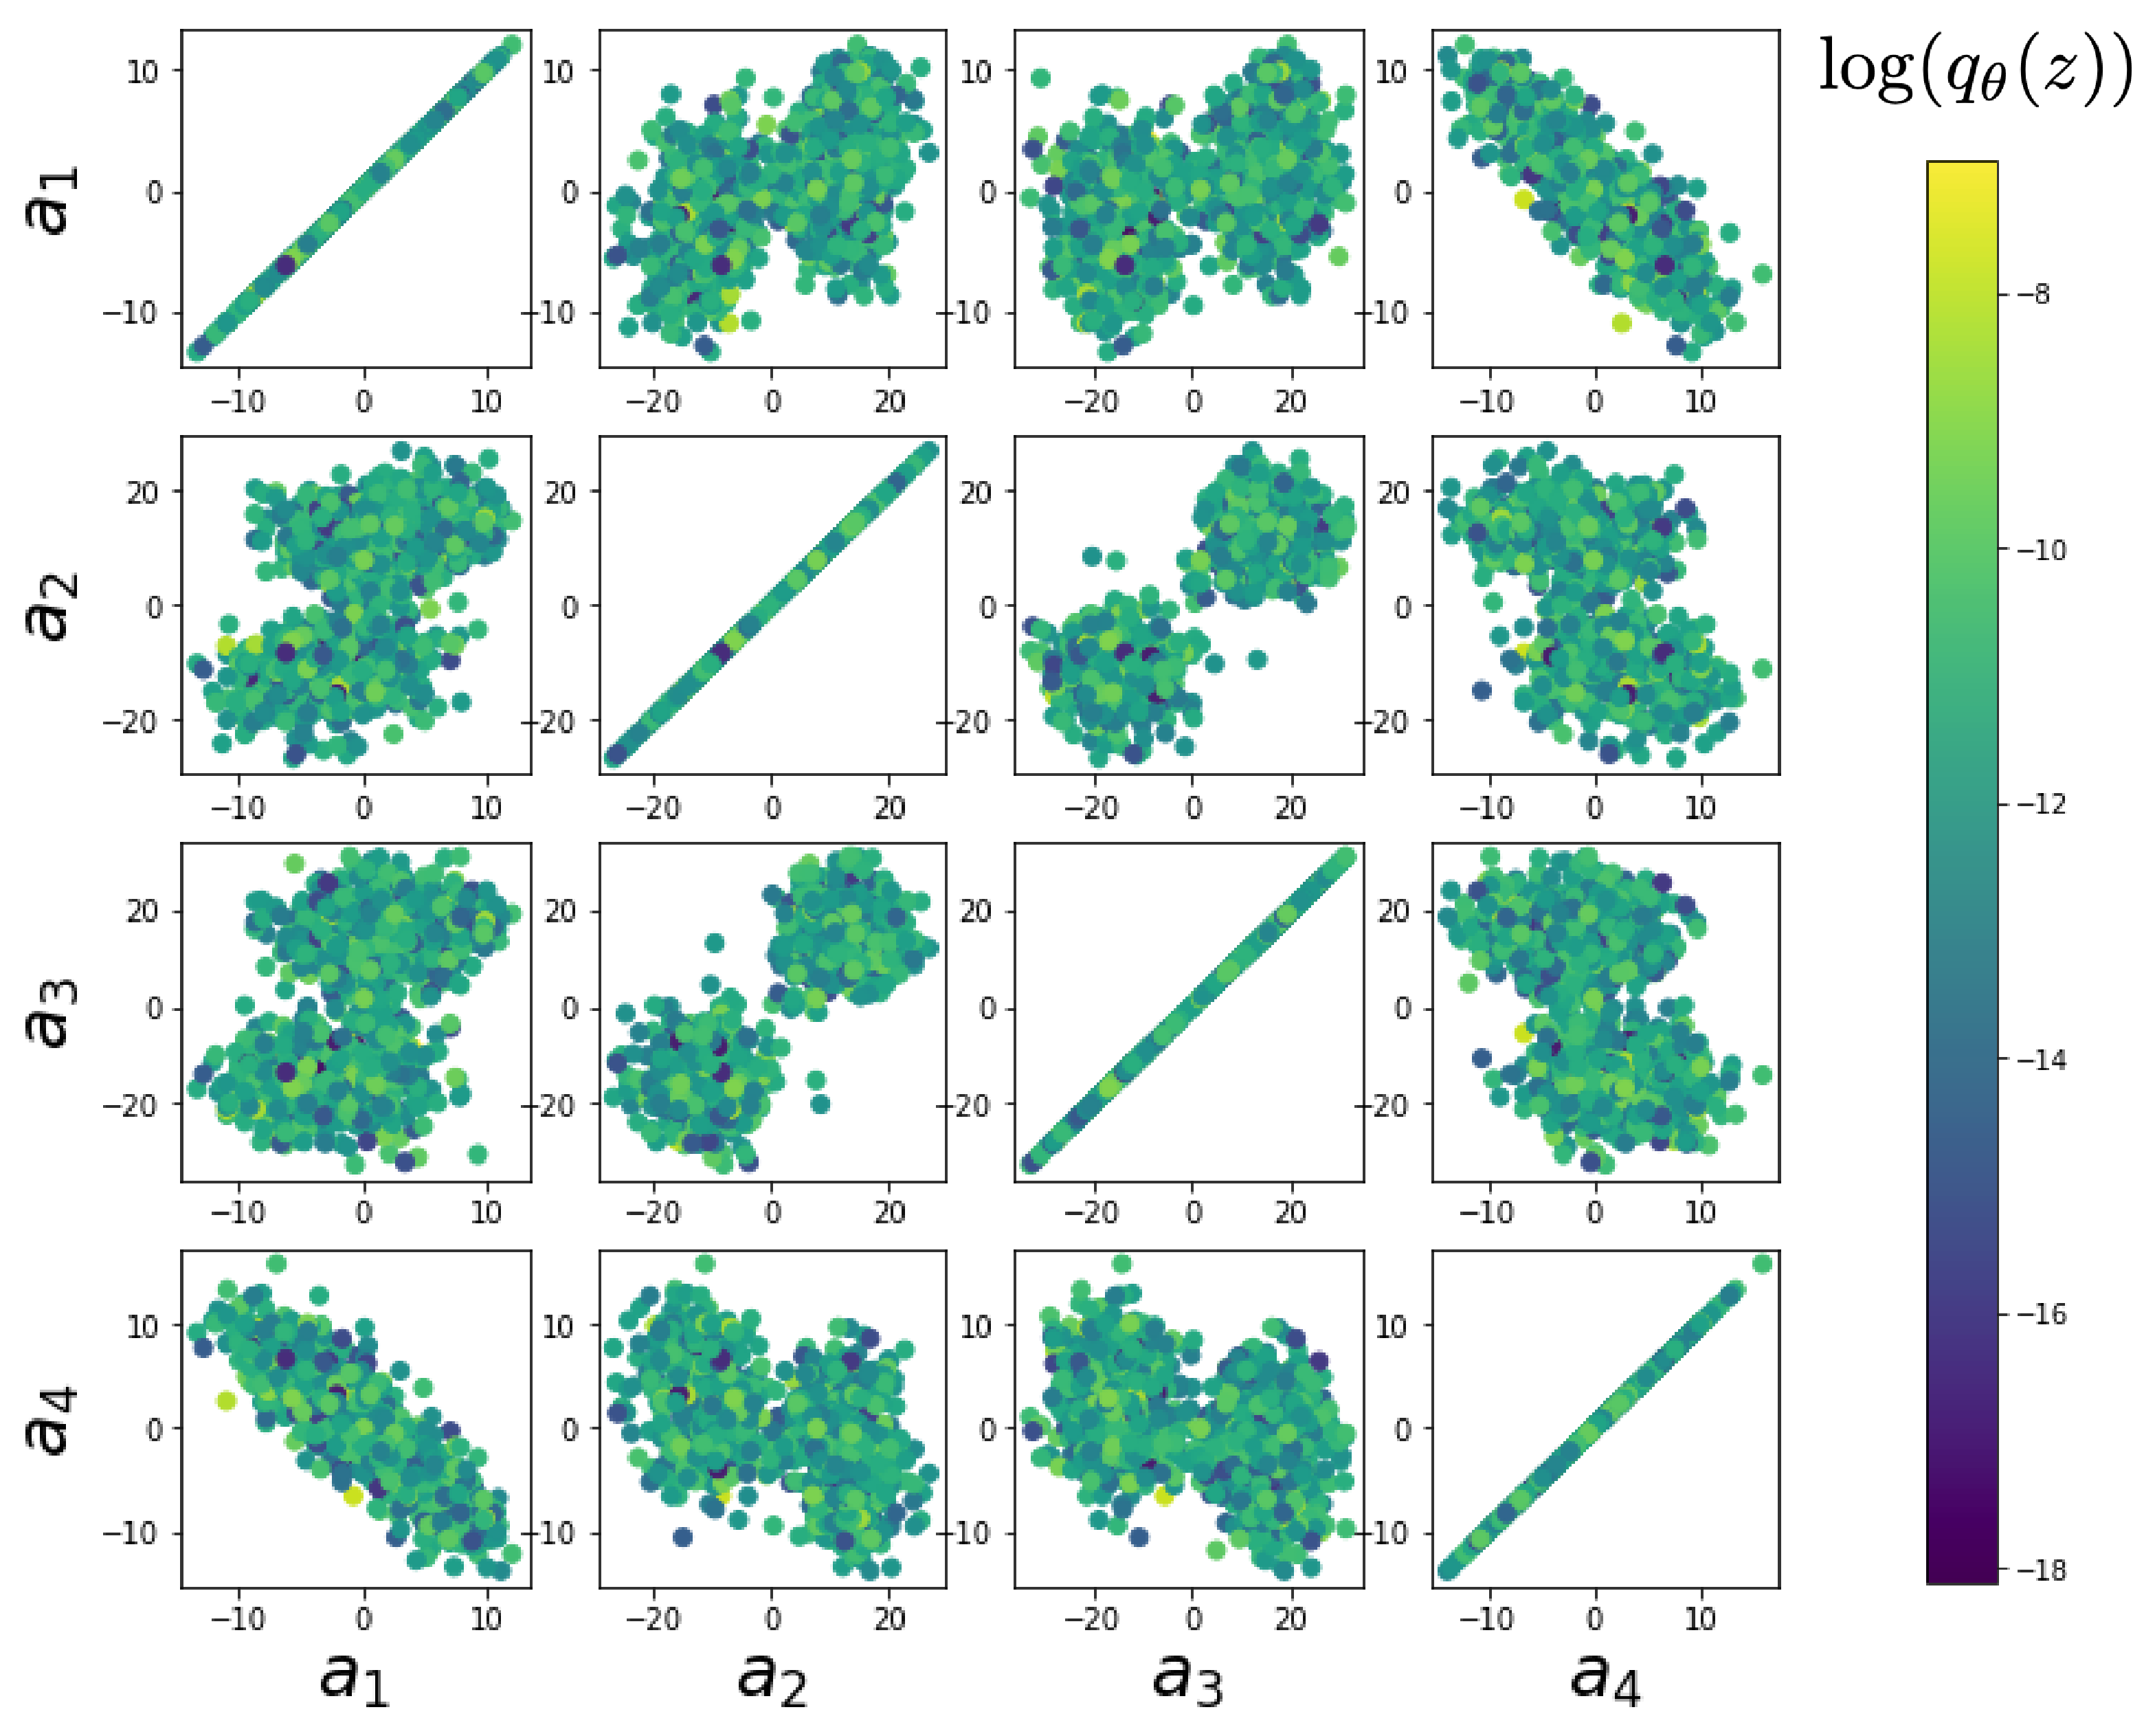
\includegraphics[scale=.3]{old_figs/appendix/Fig2.png} 
\end{center}
\vspace{-60pt}
\end{wrapfigure}
\begin{equation}
 \mu = E \begin{bmatrix} c \\ \omega \\ c^2 \\ \omega^2 \end{bmatrix} = \begin{bmatrix} 0.0 \\ 1.0 \\ 1.0 \\ 2.0 \end{bmatrix}
 \end{equation} 
We could simuilate system activity $x$ from $z$ for some finite number of time steps, and estimate $\omega$ by e.g. taking the peak of the Discrete Fourier series.  Instead, the sufficient statistics for this oscillating behavior are computed through a closed form function $f_{p, T}(z)$ by taking the eigendecomposition of the dynamics matrix
\begin{equation}
E_{x\sim p(x \mid z)}\left[T(x)\right] = f_{p,T}(z) =  \begin{bmatrix} \text{real}(\lambda_1) \\ \frac{\text{imag}(\lambda_1)}{2 \pi} \\ \text{real}(\lambda_1)^2 \\ (\frac{\text{imag}(\lambda_1)}{2 \pi})^2 \end{bmatrix}
\end{equation}
where $\lambda_1$is the eigenvalue of $\frac{1}{\tau}A$ with greatest real part.
Even though $E_{z \sim q_\theta}\left[ E_{x\sim p(x \mid z)}\left[T(x)\right] \right]$ is calculable directly via $f_{p,T}$, we cannot derive the distribution $q^*_\theta$, since the backward mapping from the mean parameters $\mu$ to the natural parameters $\eta$ of this exponential family is unknown.  Instead, we can train a DSN to learn the degenerate linear system parameterization (Fig. 2). Even this relatively simple system has nontrivial (though intuitively sensible) structure in the parameter distribution.  Indeed, more subtle model-behavior combinations will have even more complexity, further motivating DSNs. \\

\subsection{Augmented Lagrangian optimization}
To optimize $q_\theta(z)$ in equation 1, the constrained optimization is performed using the augmented Lagrangian method.  The following objective is minimized:
\begin{equation}
L(\theta; \lambda, c) = -H(q_\theta) + \lambda^\top R(\theta) + \frac{c}{2}||R(\theta)||^2
\end{equation}
where $R(\theta) = E_{z \sim q_\theta}\left[ E_{x\sim p(x \mid z)}\left[T(x) - \mu \right] \right]$, $\lambda \in \mathcal{R}^m$ are the Lagrange multipliers and $c$ is the penalty coefficient.  For a fixed $(\lambda, c)$, $\theta$ is optimized with stochastic gradient descent.  A low value of $c$ is used initially, and increased during each augmented Lagrangian epoch. Similarly, $\lambda$ is tuned each epoch based on the constraint violations.  For the linear 2-dimensional system (Fig. 2) optimization hyperparameters are initialized to $c_1 = 1.0$ and $\lambda_1 = \bf{0}$.  The penalty coefficient is updated based on a hypothesis test regarding the reduction in constraint violation.  The p-value of $E[||R(\theta_{k+1})||] > \gamma E[||R(\theta_{k})||]$ is computed, and $c_{k+1}$ is updated  to $\beta c_k$ with probability $1-p$.  Throughout the project, $\beta = 4.0$ and $\gamma = 0.25$ is used.  The other update rule is $\lambda_{k+1} = \lambda_k + c_k \frac{1}{n} \sum_{i=1}^n (T(x^{(i)}) - \mu)$.  Each augmented Lagrangian epoch runs for 50,000 iterations.  We consider the optimization to have converged when a null hypothesis test of constraint violations being zero is accepted for all constraints at a significance threshold 0.05.  This is the dotted line on the plots below depicting the optimization cutoff of the DSN optimization for the 2-dimensional linear system.  If the optimization is left to continue running, entropy may decrease, and structural pathologies in the distribution may be introduced.

\begin{figure}
  \begin{center}  
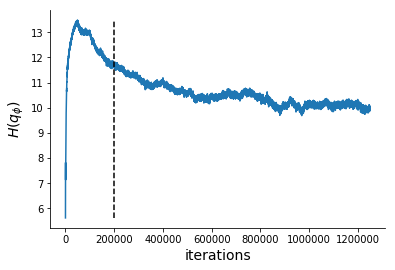
\includegraphics[scale=.3]{old_figs/appendix/linear2D_H_opt.png} \\
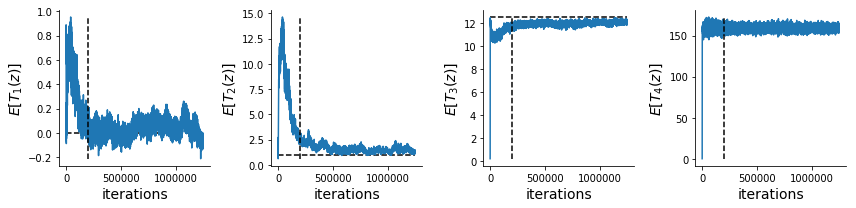
\includegraphics[scale=.4]{old_figs/appendix/linear2D_constraints_opt.png} 
\end{center}
 \caption{\label{fig:figS1} 2D linear system DSN optimization.  (Top) entropy. (Bottom) Constraint errors. }
 \end{figure}
 
 If the deep generative model parameters $\theta$ are randomly initialized,the intention is that $c$ and $\lambda$ start at values encouraging entropic growth early in optimization.  Then, as they increase in magnitude with each training epoch, the constraint satisfaction terms are increasingly weighted, resulting in a decrease in entropy.  Rather than using a naive initialization, before the DSN training, we otpimize the density network parameters to generate samples of an isotropic gaussian of a selected variance, such as 1.0 for the linear 2-D DSN training depicted in Figs. 2 and 3.  This provides a convenient starting point, whose level of entropy is controlled by the user.


\subsection{Model comparison and revision}
Bayesian statistical analyses allow us to make inferences about the rules that govern the data we have and will have, which is commonly framed as inductive reasoning. As Gelman and Shalizi remind us \cite{gelman2013philosophy}, model checking procedures comparing test statistics of the data and posterior predictive distribution facilitate model rejection through hypothetico-deductive reasoning. Recently, more attention has been given to making such hypothetico deductive statements in population-level neuroscience \cite{elsayed2017structure}.  Akin to these practices, we can compare full distributions of test statistics of models $\mathcal{M}_{p,\mathcal{B}}$ indexed by generative model $p$ and produced behavior $\mathcal{B}$ with DSNs.  Such testing can be done while keeping the model consistent, the behavior consistent, or changing both model and behavior.  Critically, none of the listed types of model comparisons directly relies on collected data as is typical in traditional statistical thinking. While the behaviors we are interested in are likely motivated by data collected through experimentation, the data itself is unnecessary for making hypothetico-deductive statements about the relative characteristics of models producing such behaviors.

Access to the full probabilistic degenerate solution space of a theoretical model that yields accurate postdictions can inform model revision in several ways. Say we have behaviors $\mathcal{B}_1$ and $\mathcal{B}_2$, which are well established experimentally.  We have some model $p(x \mid z; \phi)$ with parameters $z$ and hyperparameters governing model selection $\phi$, which is capable of producing behaviors $\mathcal{B}_1$ and $\mathcal{B}_2$ independently.  We break down $\phi = \left[\phi_c, \phi_{nc}\right]$, into continuous and non-continuous sets of model selction parameters, respectfully.  For example, $\phi_{nc}$ may govern some choice of model architecture.  If we learn a DSN for $\mathcal{M}_{p,\mathcal{B}}$  and find there is no support of $q^*_\theta(z)$ that yields $\mathcal{B}_2$, we effectively realize that our model is wrong. Our first step for model revision can be to choose some subset of $\phi_{c,opt} \subseteq \phi_c$, and concatenate it to $z$ so that $\tilde{z} = \left[z, \phi_{c, opt}\right]$ with $\tilde{\phi} = \left[\phi_{c,fixed}, \phi_{nc} \right]$, and learn a new DSN $\mathcal{M}_{\tilde{p}, \mathcal{B}_1}$ for generative model $\tilde{p}(x \mid \tilde{z}, \tilde{\phi})$.  Then, we can look for $\phi_{c,opt}$ that yield $\mathcal{B}_2$ indicating the necessary model revision. Alternatively, insights from the probabilistic degenerate solution space can give theorists with specialty knowledge about $p(x \mid z; \phi)$ information on how to change $\phi$ in general.


\subsection{Neuron-type population responses in primary visual cortex (V1)}
\subsubsection{Model}
4-neuron V1 circuit.

This is the standard 4-neuron rate model of V1 activity consisting of
\begin{itemize}
\item E: pyramidal (excitatory) neurons
\item P: parvalbumim expressing inhibitory neurons
\item S: somatostatin expressing inhibitory neurons
\item V: vasoactive intestinal peptide (VIP) expressing inhibitory neurons
\end{itemize}

The dynamics of each neural populations average rate
$r = \begin{bmatrix} r_E \\ r_P \\ r_S \\ r_V \end{bmatrix}$
are given by:
\begin{equation}
\tau \frac{dr}{dt} = -r + [Wr + h]_+^n
\end{equation}

In some cases, these neuron types do not send projections to one of the other
types.  Additionally, much work, such as \cite{pfeffer2013inhibition}
has been done to measure the relative magnitudes of the synaptic projections
between neural types.
\begin{equation}
W = \begin{bmatrix} W_{EE} & -1.0 & -0.54 & 0 \\ W_{PE} & -1.01 & -0.33 & 0 \\ W_{SE} & 0 & 0 & -0.15 \\ W_{VE} & -0.22 & -0.77 & 0 \end{bmatrix}
\end{equation}

In this model, we are interested in capturing V1 responses across varying
contrasts $c$, stimulus sizes $s$, and locomotion $r$ conditions as
in \cite{dipoppa2018vision}.

\begin{equation}
h = b + g_{FF}(c) h_{FF} + g_{LAT}(c,s) h_{LAT} + g_{RUN}(r) h_{RUN}
\end{equation}

\begin{equation} \begin{bmatrix} h_E \\ h_P \\ h_S \\ h_V \end{bmatrix}
 = \begin{bmatrix} b_E \\ b_P \\ b_S \\ b_V \end{bmatrix} + g_{FF}(c) \begin{bmatrix} h_{FF,E} \\ h_{FF,P} \\ 0 \\ 0 \end{bmatrix} + g_{LAT}(c,s) \begin{bmatrix} h_{LAT,E} \\ h_{LAT,P} \\ h_{LAT,S} \\ h_{LAT,V} \end{bmatrix} + g_{RUN}(r) \begin{bmatrix} h_{RUN,E} \\ h_{RUN,P} \\ h_{RUN,S} \\ h_{RUN,V} \end{bmatrix}
\end{equation}

where $g_{FF}(c)$, $g_{LAT}(c,s)$, and $g_{FF}(r)$ modulate the input
parmeterization $h$ according to condition. 

The two options for $g_{FF}$ in the code are: \\
``c" (default) - $g_{FF}(c) = c$ \\
``saturate" - $g_{FF}(c) = \frac{c^a}{c_{50}^a + c^a}$ \\

The two options for $g_{LAT}$ in the code are: \\
``linear" (default) - $g_{LAT}(c, s) = c\left[ s - s_0 \right]$ \\
``square" - $g_{LAT}(c, s) = c\left[ s^2 - s_0^2 \right]_+$ \\

The two options for $g_{RUN}$ in the code are: \\
``r" (default) - $g_{RUN}(r) = r$ \\

\subsubsection{Characterizing behavior}
\begin{equation}
  d_{\alpha,ss} = r_{\alpha,ss}(c_2,s_2,r_2) - r_{\alpha,ss}(c_1,s_1,r_1)
 \end{equation}

The total constraint vector is
\begin{equation}
  E_{x\sim p(x \mid z)}\left[T(x)\right] = \begin{bmatrix} d_{E,ss} \\ d_{P,ss} \\ d_{S,ss} \\ d_{V,ss} \\ d_{E,ss}^2 \\ d_{P,ss}^2 \\ d_{S,ss}^2 \\ d_{V,ss}^2 \end{bmatrix}
\end{equation}

\subsection{Information routing in the superior colliculus (SC)}
\subsubsection{Background}
Task: Cue indicates Pro or Anti condition.  Following a delay after the cue, the mouse is supposed to lick right/left if the light stimulus is on the right/left in the Pro condition, and left/right in the Anti condition.  

Electrophysiological recordings from SC and PFC indicate a much stronger encoding of task context in SC than PFC, and a significantly earlier representation of choice than PFC.  This is discordant with the prevailing understanding that PFC sends the output of flexible routing to SC.

SC neurons can be succinctly sorted into two groups -- cue neurons and delay/choice neurons by the period (before and after cue removal, respectively) of the task in which they strongly encode task context.  Furthermore, these delay/choice neurons have relatively distorted representations of task context on error trials.

There was a surprisingly high fidelity match between Pro-tuned neurons and Contra-response-tuned neurons, and between Anti-tuned neurons and Ipsi-response-tuned neurons.

During bilateral SC silencing experiments, performance was unnaffected during task cue and choice period silencing.  In delay period inactivation experiments, only performance in the Anti condition was reduced significantly.

\subsubsection{Model}
\begin{wrapfigure}{h}{.5\textwidth}
\vspace{-.8cm}
 \caption{\label{fig:fig3} SC model from (Duan et al. 2019).}
  \begin{center}  
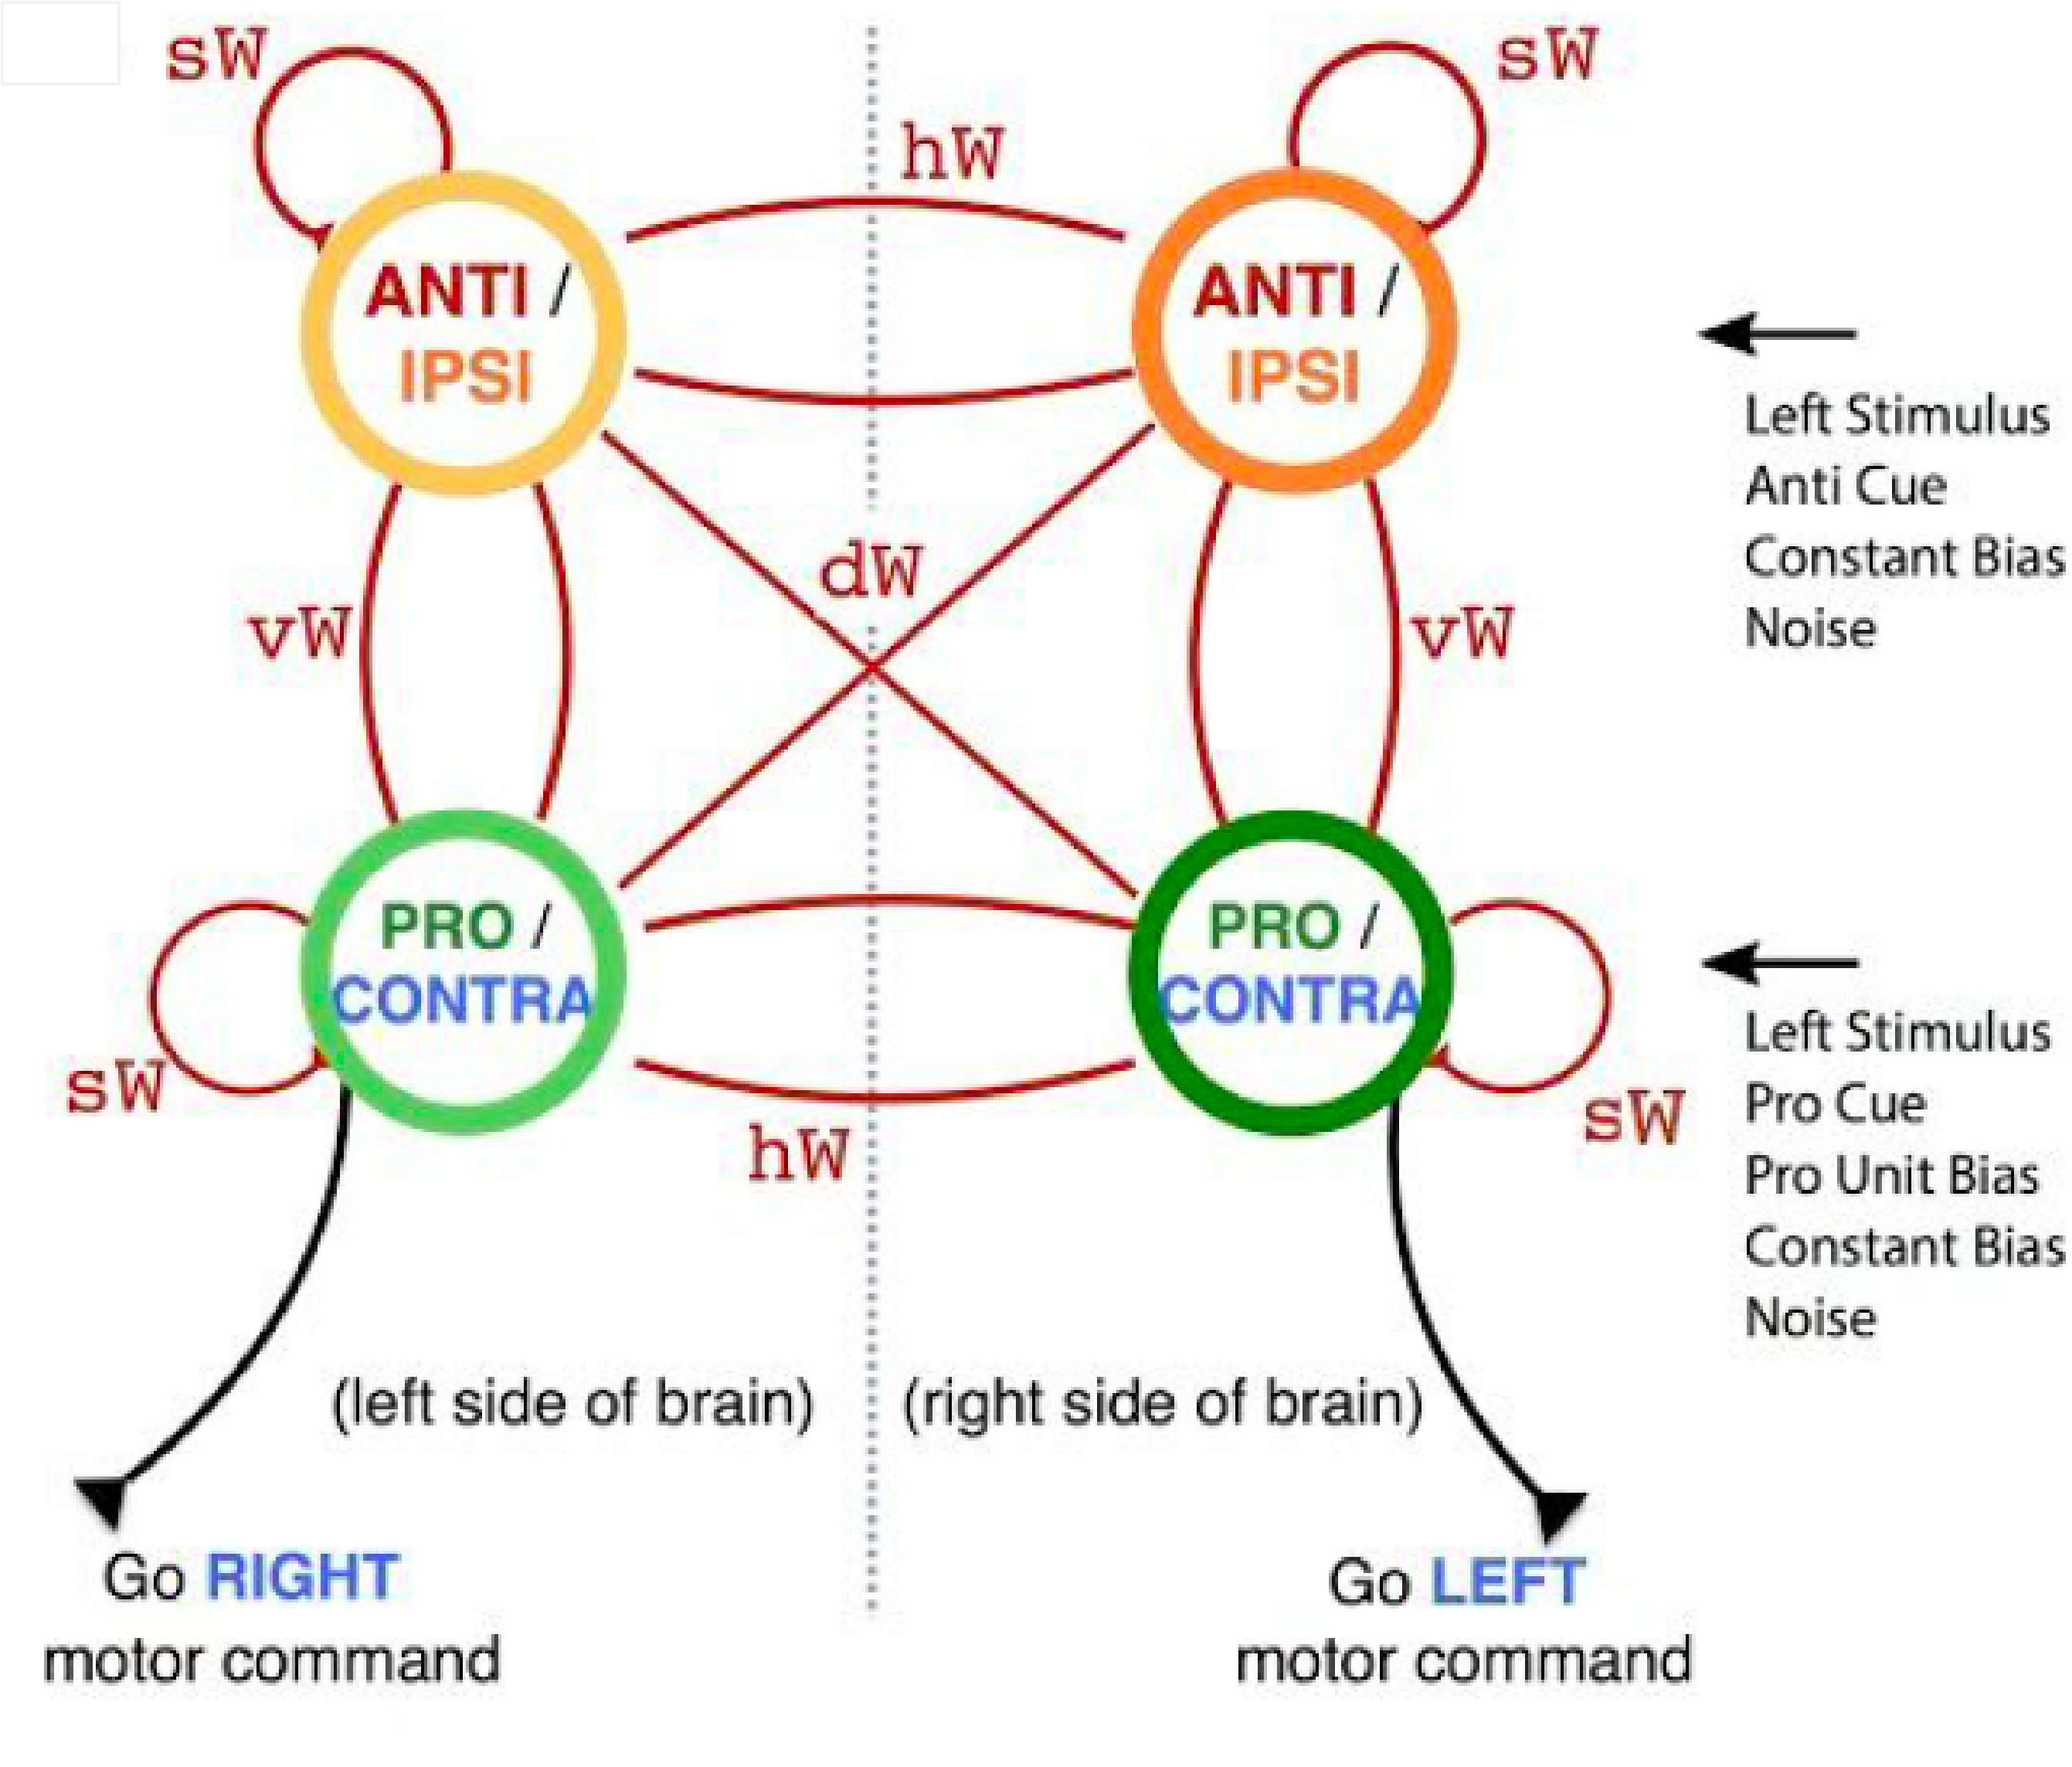
\includegraphics[scale=.3]{old_figs/fig4/Duan_2019_Fig6_clean.png} 
\end{center}
\end{wrapfigure}
The authors designed a nonlinear dynamical model of SC (Fig. 3) and found parameterizations which yielded a high-level description of these experimental results.

There are four total units: two in each hemisphere corresponding to the PRO/CONTRA and ANTI/IPSI populations.  Each unit had an external ($V_i$) and internal ($U_i$) variable related by
\begin{equation}
V_i(t) =\eta(t)\left(\frac{1}{2}\tanh\left(\frac{U_i(t) - \theta}{\beta}\right)+ \frac{1}{2} \right)
\end{equation}
$\theta = 0.05$ and $\beta = 0.5$ control the position and shape of the nonlinearity, repsectively, and $\eta(t)$ is the optogenetic inactivation function.

We can order the elements of $V_i$ and $U_i$ into vectors $v$ and $u$ with elements
\begin{equation}
v = \begin{bmatrix} V_{LP} \\ V_{LA} \\ V_{RP} \\ V_{RA} \end{bmatrix} \hspace{2cm} u = \begin{bmatrix} U_{LP} \\ U_{LA} \\ U_{RP} \\ U_{RA} \end{bmatrix}
\end{equation}

 The internal variables follow dynamics:
\begin{equation}
\tau \frac{\partial u}{\partial t} = -u + Wv + I + \sigma \partial W
\end{equation}
with time constant $\tau = 0.09s$ and gaussian noise $\sigma \partial W$ controlled by the magnitude of $\sigma$.  The weight matrix has 8 parameters $sW_P$, $sW_A$, $vW_{PA}$, $vW_{AP}$, $hW_P$, $hW_A$, $dW_{PA}$, and $dW_{AP}$,  related to the depiction in Fig. 2:
\begin{equation}
W = \begin{bmatrix} sW_P & vW_{PA} & hW_P & dW_{PA}  \\ vW_{AP}  & sW_A & dW_{AP}  & hW_A \\ hW_P & dW_{PA}  & sW_P & vW_{PA}  \\ dW_{AP}  & hW_A & vW_{AP}  & sW_A \end{bmatrix}
\end{equation}

The input is a sum of five constant scalar parameters:
\begin{equation}
I = I_{\text{constant}} + I_{\text{pro-bias}} + I_{\text{rule}} + I_{\text{choice-period}} + I_{\text{light}}
\end{equation}

\subsubsection{Characterizing behavior}
We are interested in finding model parameterizations, which yield high accuracy in Pro trials across no inacitviation (NI), delay period inactivation (DI), and choice period inactivation (CI).  Additionally, we want high accuracy on Anti trials during NI and CI, but low accuracy during DI.

In the manuscript, this was done by training SC models for many parameterizations, and keeping track of the parameterizations that yielded the task performance just described.  This procedure gives us a set of satisfactory parameterizations, which can be analyzed and examined to gain an understanding of the parameterizations that produce these results and the different possibilities of response types.  

With DSNs, we can use machine learning to find a maximally expansive distribution of such model parameterizations that produce the desired task responses.  This distribution on parameterizations gives us additional insight to the structure of the degenerate space of parameters that produces those task responses.  DSNs  facilitate complementary analyses for understanding the implications of all SC models that produce these responses.

Let $V_\alpha,{\text{ss}} = V_\alpha(t = 1.85)$ be the activity of neuron type $\alpha \in \left[LP, LA, RP, RA \right]$ (ss means steady-state), where we have a 1.2 second cue + delay period and a 0.65s choice period.  We want $p_{a,b}$ probability of success ($a \in \left[P, A \right]$ and $b \in \left[NI, DI, CI \right]$), with strong responses -- high or low activity when either succeeding or failing.  In the trained networks of Duan et al. 2019, this either high-or-low response type is encouraged by using term $C_2$ of the cost function (methods of Duan et al. 2019).  With DSNs, we can require that the responses approximately have the properties of Bernoulli variables (which are all or none with some rate).

For a given parameter vector sample $z_i$ from the DSN, let's consider M frozen noise realizations $\sigma \partial W_j \sim \mathcal{N}(0, \sigma) \in \mathcal{R}^T$, where $T = \text{int}(\frac{1.85}{\partial t = 0.024})$.  To encourage the steady state responses of the left and right PRO/CONTRA neurons across the various task conditions to behave as Bernoulli variables, we can ask that for the pro condition with stimulus $s \in \left[L, R\right]$:
\[ E_{\sigma \partial W} \left[ V_{LP,\text{ss}} \mid s=L, b, z_i \right] = \frac{1}{M}\sum_{j=1}^M V_{LP,\text{ss}}(s=L, b, z_i, \sigma \partial W_j) =  p_{P, b} \]
\[ E_{\sigma \partial W} \left[ V_{LP,\text{ss}} \mid s=R, b, z_i \right] = 1 - p_{P, b} \]
\[ E_{\sigma \partial W} \left[ V_{RP,\text{ss}} \mid s=L, b, z_i \right] = 1 - p_{P, b} \]
\[ E_{\sigma \partial W} \left[ V_{RP,\text{ss}} \mid s=R, b, z_i \right] = p_{P, b} \]
$Var_{\sigma \partial W}(V_{LP,\text{ss}} \mid s=L, b, z_i) =   Var_{\sigma \partial W}(V_{LP,\text{ss}} \mid s=R, b, z_i) = Var_{\sigma \partial W}(V_{RP,\text{ss}} \mid s=L, b, z_i) = $ \\
$Var_{\sigma \partial W}(V_{RP,\text{ss}} \mid s=R, b, z_i) = p_{P, b}(1 -  p_{P,b})$

and the analagous equations for the ANTI condition.  As a reminder a Bernoulli random variable $x \in \left[0, 1 \right]$ with parameter $p$ has $E\left[x \right] = p$ and $Var(x) = p(1-p)$.

DSNs enforce statistics in expectation of samples $z_i \sim q_\theta(z_i)$ from the DSN.  So we will end up imposing constraints on the vector:
\begin{equation}
E_{z \sim q_\theta(z)}
\begin{bmatrix}
E_{\sigma \partial W} \left[ V_{LP,\text{ss}} \mid s=L, b, z \right] \\
E_{\sigma \partial W} \left[ V_{LP,\text{ss}} \mid s=R, b, z \right] \\
E_{\sigma \partial W} \left[ V_{RP,\text{ss}} \mid s=L, b, z \right] \\
E_{\sigma \partial W} \left[ V_{RP,\text{ss}} \mid s=R, b, z \right] \\
Var_{\sigma \partial W} \left[ V_{LP,\text{ss}} \mid s=L, b, z \right] \\
Var_{\sigma \partial W} \left[ V_{LP,\text{ss}} \mid s=R, b, z \right] \\
Var_{\sigma \partial W} \left[ V_{RP,\text{ss}} \mid s=L, b, z \right] \\
Var_{\sigma \partial W} \left[ V_{RP,\text{ss}} \mid s=R, b, z \right] \\
... \\
\end{bmatrix}
 = \begin{bmatrix}
p_{P, b} \\
1 - p_{P, b} \\
1 - p_{P, b} \\
p_{P, b} \\
p_{P, b}(1 - p_{P, b}) \\
p_{P, b}(1 - p_{P, b}) \\
p_{P, b}(1 - p_{P, b}) \\
p_{P, b}(1 - p_{P, b}) \\
... \\ 
\end{bmatrix}
\end{equation}

We can additionally control the variance across samples $z$ of these statistics using second moment constraints in addition to the first moment. 

\subsection{Context-dependent decision making in a low-rank RNN}
\subsubsection{Background}
Mean field theory (MFT) originated as a useful tool for physicists studying many-body problems, particularly interactions of many particles in proximity.  Deriving an equation for the probability of configurations of such systems of particles in equilibrium requires a partition function, which is essentially the normalizing constant of the probability distribution.  The partition function relies on the Hamiltonian, which is an expression for the total energy of the system.  Many body problems in physics are usually pairwise interaction models, resulting in  combinatoric growth issue in the calculation of the Hamiltonian.  A mean field assumption that some degrees of freedom of the system have independent probabilities makes approximations to the Hamilton tractable.  Importantly, when minimizing the free energy of the system (to find the equilibrium state), the mean field assumption allows the derivation of consistency equations.  For a given system parameterization, we can solve the consistency equations using an off-the-shelf nonlinear system of equations solver.

Using the same modeling strategy as MFT, physicists developed dynamic mean field theory (DMFT) to describe dynamics of macroscopic spin glass properties. Later, this same formalism was used to describe dynamic properties of unstructured neural networks (Somp ’88).

\subsubsection{Model}
The network dynamics of neuron $i$'s rate $x$ evolve according to:
\begin{equation}
\dot{x}_i(t) = -x_i(t) + \sum_{j=1}^N J_{ij} \phi(x_j(t)) + I_i 
\end{equation}
where the connectivity is comprised of a random and structured component:
\begin{equation}
J_{ij} = g \chi_{ij} + P_{ij}
\end{equation}
The random all-to-all component has elements drawn from
$\chi_{ij} \sim \mathcal{N}(0, \frac{1}{N})$, and the structured
component is a sum of $r$ unit rank terms:
\begin{equation}
P_{ij} = \sum_{k=1}^r \frac{m_i^{(k)}n_j^{(k)}}{N}
\end{equation}
We use this theory to compute $T(x)$ when training DSNs to learn maximum entropy distributions of network connectivities that solve a task.  While the theory is currently used to design low-rank solutions to tasks, we are able to learn the full distribution of low-rank RNN parameterizations that solve a given task.

\subsubsection{Characterizing behavior}
\textbf{DMFT solvers}

\textbf{Rank 1 sponatneous stationary solutions} \\
Rank-1 vectors $m$ and $n$ have elements drawn
\[m_i \sim \mathcal{N}(M_m, \Sigma_m)\]
\[n_i \sim \mathcal{N}(M_n, \Sigma_n)\]

\textbf{Parameters:} \\
\[z = \begin{bmatrix} g & M_m & M_n & \Sigma_m \end{bmatrix}^\top \]

\textbf{Consistency equations:} (eq 83 of M \& O) \\\begin{equation}
\begin{split}
\mu = M_m M_n \langle \left[ \phi_i \right] \rangle := F(\mu, \Delta_0) \\
\Delta_0 = g^2 \langle \left[ \phi_i^2 \right] \rangle + \Sigma_m^2 M_n^2 \langle \left[ \phi_i \right] \rangle^2 := G(\mu, \Delta_0)
\end{split}
\end{equation}

\textbf{Solver:} \\
\begin{equation}
\begin{split}
\dot{\mu}(t) = -\mu(t) + F(\mu(t), \Delta_0(t)) \\
\dot{\Delta_0}(t) = -\Delta_0(t) + G(\mu(t), \Delta_0(t))
\end{split}
\end{equation}

\textbf{Rank1 sponatneous chaotic solutions} \\
Rank-1 vectors $m$ and $n$ have elements drawn
\[m_i \sim \mathcal{N}(M_m, \Sigma_m)\]
\[n_i \sim \mathcal{N}(M_n, \Sigma_n)\]

\textbf{Parameters:} \\
\[z = \begin{bmatrix} g & M_m & M_n & \Sigma_m \end{bmatrix}^\top \]

\textbf{Consistency equations:} (eq 86 of M \& O) \\
\begin{equation}
\begin{split}
 \mu = F(\mu, \Delta_0, \Delta_\infty) = M_m M_n \int \mathcal{D}z \phi(\mu + \sqrt{\Delta_0} z) \\
\Delta_0 = G(\mu, \Delta_0, \Delta_\infty) = [\Delta_\infty^2 + 2g^2\{\int \mathcal{D}z \Phi^2(\mu + \sqrt{\Delta_0}z)  \\
- \int \mathcal{D}z [\int \mathcal{D}x \Phi(\mu + \sqrt{\Delta_0 - \Delta_\infty}x + \sqrt{\Delta_\infty}z)]^2\} +M_n^2 \Sigma_m^2 \langle[\phi_i]\rangle^2(\Delta_0 - \Delta_\infty)]^{\frac{1}{2}} \\
\Delta_\infty = H(\mu, \Delta_0, \Delta_\infty) = g^2 \int \mathcal{D}z \left[ \int \mathcal{D}x \Phi(\mu + \sqrt{\Delta_0 - \Delta_\infty} + \sqrt{\Delta_\infty}z \right]^2 + M_n^2 \Sigma_m^2 \langle [\phi_i] \rangle^2
\end{split}
\end{equation}

\textbf{Solver:} \\
\begin{equation}
\begin{split}
\dot{\mu}(t) = -\mu(t) + F(\mu(t), \Delta_0(t), \Delta_\infty(t)) \\
\dot{\Delta_0}(t) = \Delta_0(t) + G(\mu(t), \Delta_0(t), \Delta_\infty(t)) \\
\dot{\Delta_\infty}(t) = -\Delta_\infty(t) + H(\mu(t), \Delta_0(t), \Delta_\infty(t))
\end{split}
\end{equation}

\textbf{Rank 1 with input chaotic solutions} \\
Rank-1 vectors $m$ and $n$ have elements drawn
\[m_i \sim \mathcal{N}(M_m, \Sigma_m)\]
\[n_i \sim \mathcal{N}(M_n, \Sigma_n)\]
The current has the following statistics:
\[I = M_I + \frac{\Sigma_{mI}}{\Sigma_m}x_1 + \frac{\Sigma_{nI}}{\Sigma_n}x_2 + \Sigma_\perp h\]
where $x_1$, $x_2$, and $h$ are standard normal random variables.

\textbf{Parameters:} \\
\[z = \begin{bmatrix} g & M_m & M_n & M_I & \Sigma_m & \Sigma_n & \Sigma_{mI} & \Sigma_{nI} & \Sigma_\perp \end{bmatrix}^\top \]

(expansion of 98 of M \& O) \\
The $\ddot{\Delta}$ equation is broken into the equation for $\Delta_0$ and $\Delta_\infty$ by the autocorrelation dynamics assertions.
\[\ddot{\Delta(\tau)} = - \frac{\partial V}{\partial \Delta} \]
\[\ddot{\Delta} = \Delta - \lbrace g^2 \langle \left[ \phi_i(t) \phi_i(t + \tau) \right] \rangle + \Sigma_m^2 \kappa^2 + 2\Sigma_{mI} \kappa + \Sigma_I^2 \rbrace \]

We can write out the potential function by integrating the negated RHS.
\[V(\Delta, \Delta_0) = \int \mathcal{D} \Delta \frac{\partial V(\Delta, \Delta_0)}{\partial \Delta}\]
\[V(\Delta, \Delta_0) = -\frac{\Delta^2}{2} + g^2 \langle \left[ \Phi_i(t) \Phi_i(t + \tau) \right] \rangle + (\Sigma_m^2 \kappa^2 + 2\Sigma_{mI} \kappa + \Sigma_I^2)\Delta + C \]
 

We assume that as time goes to infinity, the potential relaxes to a steady state.
\[\frac{\partial V(\Delta_\infty, \Delta_0)}{\partial \Delta}  = 0 \]
\[\frac{\partial V(\Delta_\infty, \Delta_0)}{\partial \Delta} = - \Delta + \lbrace g^2 \langle \left[ \phi_i(t) \phi_i(t + \infty) \right] \rangle + \Sigma_m^2 \kappa^2 + 2\Sigma_{mI} \kappa + \Sigma_I^2 \rbrace = 0\]
\[\Delta_\infty = g^2 \langle \left[ \phi_i(t) \phi_i(t + \infty) \right] \rangle + \Sigma_m^2 \kappa^2 + 2\Sigma_{mI} \kappa + \Sigma_I^2 \]
\[\Delta_\infty = g^2 \int \mathcal{D}z \left[ \int \mathcal{D}x \phi(\mu + \sqrt{\Delta_0 - \Delta_\infty}x + \sqrt{\Delta_\infty}z \right]^2 + \Sigma_m^2 \kappa^2 + 2\Sigma_{mI} \kappa + \Sigma_I^2 \]

Also, we assume that the energy of the system is perserved throughout the entirety of its evolution. 
\[V(\Delta_0, \Delta_0) = V(\Delta_\infty, \Delta_0)\]
\[-\frac{\Delta_0^2}{2} + g^2 \langle \left[ \Phi_i(t) \Phi_i(t) \right] \rangle + (\Sigma_m^2 \kappa^2 + 2\Sigma_{mI} \kappa + \Sigma_I^2)\Delta_0 + C = -\frac{\Delta_\infty^2}{2} + g^2 \langle \left[ \Phi_i(t) \Phi_i(t) \right] \rangle + (\Sigma_m^2 \kappa^2 + 2\Sigma_{mI} \kappa + \Sigma_I^2)\Delta_\infty + C   \]
\[\frac{\Delta_0^2-\Delta_\infty^2}{2} = g^2 \left( \langle \left[ \Phi_i(t) \Phi_i(t) \right] \rangle - \langle \left[ \Phi_i(t) \Phi_i(t) \right] \rangle \right) + (\Sigma_m^2 \kappa^2 + 2\Sigma_{mI} \kappa + \Sigma_I^2)(\Delta_0-\Delta_\infty)\]

\[\frac{\Delta_0^2-\Delta_\infty^2}{2} = g^2 \left( \int \mathcal{D}z \Phi^2(\mu + \sqrt{\Delta_0}z) - \int \mathcal{D}z \int \mathcal{D}x \Phi(\mu + \sqrt{\Delta_0 - \Delta_\infty}x + \sqrt{\Delta_\infty}z)  \right) \] 
\[+ (\Sigma_m^2 \kappa^2 + 2\Sigma_{mI} \kappa + \Sigma_I^2)(\Delta_0-\Delta_\infty)\]

\textbf{Consistency equations:} \\ 
\begin{equation}
\begin{split}
\mu = F(\mu, \kappa, \Delta_0, \Delta_\infty) = M_m \kappa + M_I \\
\kappa = G(\mu, \kappa, \Delta_0, \Delta_\infty) = M_n \langle \left[ \phi_i \right] \rangle + \Sigma_{nI} \langle \left[ \phi_i' \right] \rangle \\
\frac{\Delta_0^2-\Delta_\infty^2}{2} = H(\mu, \kappa, \Delta_0, \Delta_\infty) = g^2 \left( \int \mathcal{D}z \Phi^2(\mu + \sqrt{\Delta_0}z) - \int \mathcal{D}z \int \mathcal{D}x \Phi(\mu + \sqrt{\Delta_0 - \Delta_\infty}x + \sqrt{\Delta_\infty}z)  \right) \\
+ (\Sigma_m^2 \kappa^2 + 2\Sigma_{mI} \kappa + \Sigma_I^2)(\Delta_0-\Delta_\infty) \\
\Delta_\infty = L(\mu, \kappa, \Delta_0, \Delta_\infty)  = g^2 \int \mathcal{D}z \left[ \int \mathcal{D}x \phi(\mu + \sqrt{\Delta_0 - \Delta_\infty}x + \sqrt{\Delta_\infty}z \right]^2 + \Sigma_m^2 \kappa^2 + 2\Sigma_{mI} \kappa + \Sigma_I^2
\end{split} 
\end{equation}

\textbf{Solver:}
\begin{equation}
\begin{split}
x(t) = \frac{\Delta_0(t)^2-\Delta_\infty(t)^2}{2} \\
\Delta_0(t) = \sqrt{2x(t) + \Delta_\infty(t)^2} \\
\dot{\mu}(t) = -\mu(t) + F(\mu(t), \kappa(t), \Delta_0(t), \Delta_\infty(t)) \\
\dot{\kappa}(t) = -\kappa + G(\mu(t), \kappa(t), \Delta_0(t), \Delta_\infty(t)) \\
\dot{x}(t) = -x(t) + H(\mu(t), \kappa(t), \Delta_0(t), \Delta_\infty(t)) \\
\dot{\Delta_\infty}(t) = -\Delta_\infty(t) + L(\mu(t), \kappa(t), \Delta_0(t), \Delta_\infty(t))
\end{split}
\end{equation}


\textbf{Integration of a noisy stimulus} \\
\textbf{Parameters:} \\
\[z = \begin{bmatrix} g & M_m & M_n & M_I & \Sigma_m & \Sigma_n & \Sigma_{mI} & \Sigma_{nI} & \Sigma_\perp \end{bmatrix}^\top \]

\textbf{Behavior:} \\
\[z = \begin{bmatrix} \kappa(M_{I,low}), \kappa(M_{I,high}), \Delta_T, \kappa(M_{I,low})^2, \kappa(M_{I,high})^2, \Delta_T^2 \end{bmatrix}^\top \]


\textbf{Rank 2 networks have the following consistency equations for $\Delta_0$ and $\Delta_\infty$} \\
\[\rho_m = \langle m_i^{(1)} m_i^{(2)} \rangle \]
\begin{equation}
\begin{split}
\frac{\Delta_0^2-\Delta_\infty^2}{2} = H(\mu, \kappa, \Delta_0, \Delta_\infty) = g^2 \left( \int \mathcal{D}z \Phi^2(\mu + \sqrt{\Delta_0}z) - \int \mathcal{D}z \int \mathcal{D}x \Phi(\mu + \sqrt{\Delta_0 - \Delta_\infty}x + \sqrt{\Delta_\infty}z)  \right) \\
+ (2 \rho_m \kappa_1 \kappa_2 + \Sigma_m^{(1)^2} \kappa_1^2 +  \Sigma_m^{(2)^2}  \kappa_2^2 + \Sigma_I^2)(\Delta_0 - \Delta_\infty) \\
\Delta_\infty = L(\mu, \kappa, \Delta_0, \Delta_\infty)  = g^2 \int \mathcal{D}z \left[ \int \mathcal{D}x \phi(\mu + \sqrt{\Delta_0 - \Delta_\infty}x + \sqrt{\Delta_\infty}z \right]^2 + 2 \rho_m \kappa_1 \kappa_2 + \Sigma_m^{(1)^2}  \kappa_1^2 +  \Sigma_m^{(2)^2}  \kappa_2^2 + \Sigma_I^2
\end{split} 
\end{equation}

\textbf{Context-dependent discrimination} \\
\[y_A \sim \mathcal{N}(0, \Sigma_{y_A}=1.2) \]
\[y_B \sim \mathcal{N}(0, \Sigma_{y_B}=1.2) \]
\[I_{A} \sim \mathcal{N}(0, \Sigma_{I_A}=1.2) \]
\[I_{B} \sim \mathcal{N}(0, \Sigma_{I_B}=1.2) \]
\[I_{ctx,A} \sim \mathcal{N}(0, \Sigma_{I_{ctx,A}}=1) \]
\[I_{ctx,B} \sim \mathcal{N}(0, \Sigma_{I_{ctx,B}}=1) \]

\[I(t) = c_A(t)I^A + c_B(t)I^B + \gamma_A I_{ctx,A} + \gamma_B I_{ctx,B}  \]
\[m^{(1)} = y_A + \rho_m I_{ctx,A} + \beta_m w \]
\[n^{(1)} = I^A + \rho_n I_{ctx,A} + \beta_n w \]
\[m^{(2)} = y_B + \rho_m I_{ctx,B} + \beta_m w \]
\[n^{(2)} = I^B + \rho_n I_{ctx,B} + \beta_n w \]
\[y(t) = \beta_m (\kappa_1 + \kappa_2) \langle \left[\phi_i' \right] \rangle \]

\[\Sigma_I = c_A(t)\Sigma_{I_A} + c_B(t)\Sigma_{I_B} + \gamma_A \Sigma_{I_{ctx,A}} +  \gamma_B \Sigma_{I_{ctx,B}} \]
\[\Sigma_m^{(1)} = \Sigma_{y_A} + \rho_m \Sigma_{I_{ctx,A}} + \beta_m \Sigma_w \]
\[\Sigma_m^{(2)} = \Sigma_{y_B} + \rho_m \Sigma_{I_{ctx,B}} + \beta_m \Sigma_w \]
\textbf{Parameters:} \\
\[z = \begin{bmatrix} g  & \rho_m & \rho_n & \beta_m & \beta_n \end{bmatrix}^\top \]

\textbf{Consistency equations:} \\ 
\begin{equation}
\begin{split}
\kappa_1(t) = F(\kappa_1(t), \kappa_2(t), \Delta_0(t), \Delta_\infty(t)) = \rho_m \rho_n \kappa_1 \langle \left[ \phi_i' \right] \rangle +\beta_m \beta_n(\kappa_1 + \kappa_2) \langle \left[ \phi_i' \right] \rangle + c_A \Sigma_I^2 + \rho_n \gamma_A \\
\kappa_2(t) = F(\kappa_1(t), \kappa_2(t), \Delta_0(t), \Delta_\infty(t)) = \rho_m \rho_n \kappa_2 \langle \left[ \phi_i' \right] \rangle +\beta_m \beta_n(\kappa_1 + \kappa_2) \langle \left[ \phi_i' \right] \rangle + c_B \Sigma_I^2 + \rho_n \gamma_B \\
 \frac{\Delta_0^2-\Delta_\infty^2}{2} = H(\mu, \kappa, \Delta_0, \Delta_\infty) = g^2 \left( \int \mathcal{D}z \Phi^2(\mu + \sqrt{\Delta_0}z) - \int \mathcal{D}z \int \mathcal{D}x \Phi(\mu + \sqrt{\Delta_0 - \Delta_\infty}x + \sqrt{\Delta_\infty}z)  \right) \\
+ ((\Sigma_w^2 + \beta_m^2)(\kappa_1^2 + \kappa_2^2) + \Sigma_I^2(c_A^2 + c_B^2) + (\rho_m \kappa_1 + \gamma_A)^2 + (\rho_m \kappa_2 + \gamma_B)^2)(\Delta_0 + \Delta_\infty) \\
\Delta_\infty = L(\mu, \kappa, \Delta_0, \Delta_\infty)  = g^2 \int \mathcal{D}z \left[ \int \mathcal{D}x \phi(\mu + \sqrt{\Delta_0 - \Delta_\infty}x + \sqrt{\Delta_\infty}z \right]^2 + \\
(\Sigma_w^2 + \beta_m^2)(\kappa_1^2 + \kappa_2^2) + \Sigma_I^2(c_A^2 + c_B^2) + (\rho_m \kappa_1 + \gamma_A)^2 + (\rho_m \kappa_2 + \gamma_B)^2
\end{split} 
\end{equation}

\textbf{Solver:} \\
\begin{equation}
\begin{split}
x(t) = \frac{\Delta_0(t)^2-\Delta_\infty(t)^2}{2} \\
\mu = 0 \\
\Delta_0(t) = \sqrt{2x(t) + \Delta_\infty(t)^2} \\
\dot{\kappa_1}(t) = -\kappa_1 + F(\kappa_1(t), \kappa_2(t), \Delta_0(t), \Delta_\infty(t)) \\
\dot{\kappa_2}(t) = -\kappa_2 + G(\kappa_1(t), \kappa_2(t), \Delta_0(t), \Delta_\infty(t)) \\
\dot{x}(t) = -x(t) + H(\kappa_1(t), \kappa_2(t), \Delta_0(t), \Delta_\infty(t)) \\
\dot{\Delta_\infty}(t) = -\Delta_\infty(t) + L(\kappa_1(t), \kappa_2(t), \Delta_0(t), \Delta_\infty(t))
\end{split}
\end{equation}


\textbf{Behavior:} \\
\[z = \begin{bmatrix} y_1, y_2, y_3, y_4, \Delta_T, \text{sec moments...} \end{bmatrix}^\top \]


\subsection{Density network architectures}
The DSN training objective requires us to be able to compute the density of our samples, and thus the log determinant of the jacobian of each layer in our deep generative model architecture. We use density networks, which have layers called normalizing flows.  Normalizing flows are bijective functions, with relatively fast log determinant jacobian computations.

\subsubsection{Normalizing flows}
Here we mathematically describe each normalizing flow used in this paper, and how to compute its log determinant jacobian. \\\
\textbf{Planar flows} \cite{rezende2015variational}: \\
See section A.1 of \cite{rezende2015variational} for reparameterization guaranteeing invertibility.
\[f(z) = z + h(w^\top z + b)\]
\[\psi(z) = h'(w^\top z + b)w \]
\[ \left| \frac{d f(z)}{dz} \right| =  \left| 1 + u^\top \psi (z) \right| \]
We use $h = \tanh$.  The elements of $u$ and $b$ are always initialized to $0$, while the initial elements of $w$ are drawn from a glorot uniform initializer.

\textbf{Radial flows} \cite{rezende2015variational}: \\
See section A.2 of \cite{rezende2015variational} for reparameterization guaranteeing invertibility.
\[f(z) = z + \beta h(\alpha, r) (z - z_0) \]
\[ \left| \frac{d f(z)}{dz} \right| = \left[1 + \beta h(\alpha, r)\right]^{d-1} \left[ 1 + \beta h(\alpha, r) + \beta h'(\alpha, r)r) \right] \]
where $h(\alpha, r) = \frac{1}{\alpha + r}$, $r = \left| z - z_0 \right|$, and $\alpha > 0$.  A log-parameterization of $\alpha$ is used to enforce the constraint.  $\log(\alpha)$, $\beta$, and $z_0$ all have the glorot uniform initializer.

\textbf{Real NVP} \cite{dinh2016density}: \\
In a real NVP (non-volume preserving) normalizing flow, there is a sequence of ``masking" layers which parameterize bijective transformations until an output is produced.  In each ``masking" layer, a set of entries are chosen to be passed unchanged to the next masking layer.  The remaining entries are scaled and shifted by arbitrary continuous differentiable functions of the unchanged elements.

For $b \in \left[0, 1\right]^D$, let $x_{I_b}$ be the elements of arbitrary vector $x \in \mathcal{R}^D$, which have a 1 in the corresponding index of $b$.  Similarly, let $x_{I_b^C}$ be the remaining elements of $x$ (those with corresponding indices of $b$ equal to 0).  In a single masking layer of real NVP, we have the following transformation for mask $b$:
\[f(z)_{I_b} = z_{I_b}\]
\[f(z)_{I_b^C} = z_{I_b^C} \exp(s(z_{I_b})) + t(z_{I_b}) \]
Ordering the elements of $z$ such that the passed elements ($b_i=1$) are at the early indices, and letting $d = \sum_i b_i$, 
\[\frac{d f(z)}{d z} = \begin{bmatrix} \mathbb{I}_d & 0 \\ \frac{d f(z)_{I_b^C}}{d z_{I_b}} & \text{diag} (\exp \left[s(z_{I_b}) \right]) \end{bmatrix} \]
The log determinant jacobian of this masking layer is then
\[ \frac{d f(z)}{d z} = \sum_j s(z_{I_b})_j \]

The real NVP normalizing flow is constructed by a cascade of different masks.  In common practice, a mask of a particular pattern is always followed by it's complement pattern.  We adopt this pattern, and thus, our real NVP flows always have an even number of masks.  We identify masks by their number of elements - $D$, the frequency of bit flip - $f$, and state of the first element.  Below are some examples:

\begin{center}
\begin{tabular}{c | c | c | c}
D & f & first elem & mask \\
8 & 1 & 1 & $\begin{bmatrix} 1 & 1 & 1 & 1 & 0 & 0 & 0 & 0 \end{bmatrix}^\top$ \\
8 & 1 & 0 & $\begin{bmatrix} 0 & 0 & 0 & 0 & 1 & 1 & 1 & 1 \end{bmatrix}^\top$ \\
8 & 4 & 1 & $\begin{bmatrix} 1 & 0 & 1 & 0 & 1 & 0 & 1 & 0 \end{bmatrix}^\top$ \\
\end{tabular}
\end{center}

For a selection of $2k$ masks for a $D$ dimensional distribution, we use the following sequence of masks:
$f=1$, $b_1=1$ \\
$f=1$, $b_1=0$ \\
$f=\frac{D}{2}$, $b_1=1$ \\
$f=\frac{D}{2}$, $b_1=0$ \\
$f=2$, $b_1=1$ \\
$f=2$, $b_1=0$ \\
$f=\frac{D}{4}$, $b_1=1$ \\
$f=\frac{D}{4}$, $b_1=0$ \\
$f=4$, $b_1=1$ \\
$f=4$, $b_1=0$ \\
...

The parametization of functions $s$ and $t$ are $L$-layer fully-connected neural networks with $U$-units per layer.  All parameters were initialized with the glorot uniform distribution.

\textbf{Elementwise multiplication flows}: \\
\[ f(z) = a \circ z \]
\[\log (\left| \frac{d f(z)}{dz} \right|) = \sum_{i=1}^D \log (|a_i|) \]

\textbf{Shift flows}: \\
\[ f(z) = z + b \]
\[\log (\left| \frac{d f(z)}{dz} \right|) = 0\]

\subsubsection{Architectures used for each analysis}
Here, we list the architectures used in each analysis of the paper. 

\begin{center}
\begin{tabular}{c | c | c | c | c}
model & behavior & ref. & D & architecture \\
\hline
STG & 0.55 Hz & Fig. 5 & 5 & 10 planar flows, elem mult, shift  \\
V1 & loc. responses & Fig. 3 & 8 & 10 planar flows, elem mult, shift \\
SC & info routing task responses & Fig.  4 & 4 & real NVP - 4 masks, L=5, U=20 \\
rank-1 RNN & ND & Fig. 5 & 5 & 10 planar flows, elem mult, shift  \\
rank-2 RNN & CDD & Fig. 5 & 5 & 10 planar flows, elem mult, shift  \\
\end{tabular}
\end{center}




